Um die KI interaktiv zu testen, wurde eine Möglichkeit integriert, den Nao zu beeinflussen und seine Reaktion beobachten. Dabei unterscheidet man zwei Szenarien:
\begin{itemize}
\item Einen Nao durch einen zweiten, manuellen stören.
\item Einen Nao manuell in eine Situation bringen, danach die KI übernehmen lassen.
\end{itemize}

\subsection{Aufbau}
\textit{Verfasser: Schramm}\\
\\
Dazu wurde ein DecisionMaker für manuelle Steuerung implementiert. Dieser ersetzt die KI und nimmt Befehle von einem manuellen Controller entgegen.
Um eine direkte Steuerbarkeit zu gewährleisten werden einige Befehle in einer Queue gesammelt und abgearbeitet.

Neben den primären Befehlen, die in jedem Server-Zyklus abgearbeitet werden, wie zum Beispiel: Laufen, Kicken, Aufstehen … existieren auch Befehle, die parallel zu diesen ausgeführt werden können. Diese umfassen Sprechsignale und Kopfdrehungen. Sie sind in ihrer Funktion disjunkt zu den Körperbefehlen was die verwendeten Gelenke angeht. Würden diese in der Befehlsqueue ausgeführt werden, käme es zu einer Verzögerung der primären Befehle um die entsprechenden Zyklen. Deshalb werden sie in einer extra Queue für außerordentliche Befehle gesammelt und direkt vor der ordentlichen Queue ausgeführt.\\
Die zugehörigen Klassen befinden sich im Package:\\ \texttt{magma.agent.decision.simple.manual}.

\subsection{Autopiloten}
\textit{Verfasser: Schramm}\\
\\
Um die Übernahme der Kontrolle durch eine KI zu ermöglichen, werden bestehende KIs als Autopiloten eingebunden. Jeder Autopilot beinhaltet einen DecisionMaker der in regulären Bots verwendet wird. Über den manuellen Controller kann nun zwischen den Autopiloten gewechselt werden. Wird ein solcher dann aktiviert, gibt der Controller einen delegierenden Befehl an den Manuellen DecisionMaker weiter. Dieser Befehl übergibt alle Entscheidungen intern an den ihm zugeordneten KI-DecisionMaker. Somit wird der Bot von der KI übernommen. Soll zur manuellen Steuerung zurückgekehrt werden, wird der Befehl auf erledigt gesetzt und somit vom manuellen DecisionMaker aus der Queue entfernt.\\
Die verwendeten Autopiloten werden im Konstruktor übergeben. Die Auswahl erfolgt in der ComponentFactory unter \texttt{magma.agent.general}. Zur einfacheren Übersicht wurde eine Vorauswahl in einer Methode 'getAutoPilots(...)' ausgelagert.

\begin{figure}[H]
	\centering
	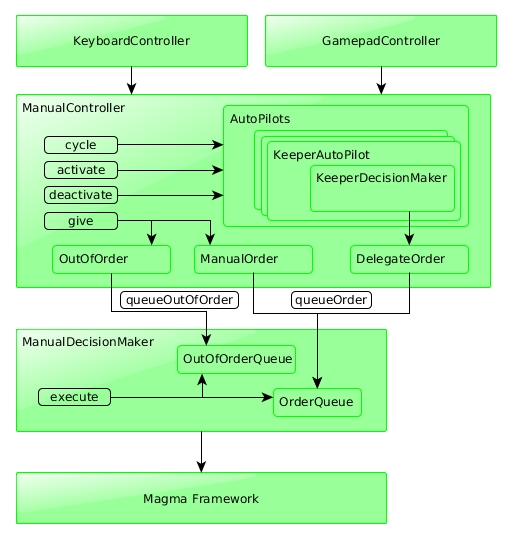
\includegraphics[width=\ScaleIfNeeded]{Grafiken/ManualCtrl/ManualDecisionMaker}
	\caption{ManualDecisionMaker}
	\label{KickMetrikAgent}
\end{figure}

\subsection{Keyboard Controller}
Eine Implementierung des Controllers stellt die Keyboardvariante dar. Dabei werden sämtliche Tastatureingaben über ein awt-Fenster abgefangen und ausgewertet. Durch drücken der Pfeiltasten lässt sich der NAO beispielsweise in die Verschiedenen Richtungen navigieren.\\
Um diesen Controller auszuwählen wird in den Startparametern die DecisionMakerID 100 übergeben.

\begin{figure}[H]
	\centering
	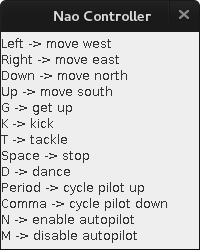
\includegraphics[width=160pt]{Grafiken/ManualCtrl/KeyboardController}
	\caption{KeyboardController - Fenster}
	\label{fig:keyboardcrtl}
\end{figure}


\subsection{Gamepad Controller}
\textit{Verfasser: Schramm}\\
\\
Für eine feinere Steuerung wurde eine Schnittstelle für Gamepads integriert. Diese bietet die selben Möglichkeiten wie über Tastatur. Dabei wurden für einige gängige Controller bereits Profile angelegt. Um diese zu erweitern und eigene hinzuzufügen, muss in der Klasse GamepadController ein neue Initialisierung angelegt werden, die das entsprechende Tastenmapping umsetzt (siehe Beispiel).\\
Um diesen Controller auszuwählen wird in den Startparametern die DecisionMakerID 101 übergeben.

\begin{lstlisting}[caption=InitializeGamePad, captionpos=b, label=lst:Gamepad]
private void initializeXBox() {
    commandMap.put("B", this::orderGetUp);
    commandMap.put("A", this::orderKick);
    commandMap.put("X", this::orderPush);
    commandMap.put("Y", this::orderStop);
    commandMap.put("Start", this::orderDance);
    commandMap.put("Right Thumb", this::cycleAutoPilotUp);
    commandMap.put("Left Thumb", this::cycleAutoPilotDown);
    commandMap.put("Mode", this::toggleAutoPilot);
    commandMap.put("Select", this::toggleEgoWalk);
    walkXComponent = Component.Identifier.Axis.X;
    walkYComponent = Component.Identifier.Axis.Y;
    lookXComponent = Component.Identifier.Axis.RX;
    lookYComponent = Component.Identifier.Axis.RY;
}
\end{lstlisting}
